\documentclass[]{article}

\usepackage[backend=biber, style=numeric]{biblatex}
\usepackage{paralist}
\usepackage{hyperref}
\usepackage{graphicx}
\usepackage{booktabs}
\usepackage{subcaption}
\usepackage{wrapfig}
\usepackage{float}

\graphicspath{ {./figures/} }
\usepackage{geometry}
\geometry{a4paper, portrait}

\addbibresource{report.bib}
\newtheorem{researchquestion}{RQ}

%opening
\title{Capita Selecta in Artificial Intelligence - Assignment 3}
\author{Arne Lescrauwaet \small(852617312) \and Joachim Verschelde \small(852594432) \and Alexander Van Hecke \small(852631385) \and Farid Rasoolzadeh Baghmisheh \small(852104522)}

\begin{document}

\maketitle

\section{Introduction} \label{sec:introduction}
This report details the step taken by Arne Lescrauwaet (852617312), Joachim Verschelde (852594432), Alexander Van Hecke (852631385) and Farid Rasoolzadeh Baghmisheh (852104522) for the third assignment of the 2023/2024 Capita Selecta in Artificial Intelligence course organised by the Open University (\cite{ou}).

For this assignment we expand on the experiments described in \cite{durability}.
In this paper, the authors investigate the use of an LLM model and a RAG setup \cite{rag} to asses company durability disclosures.
By examining published sustainability reports of carbon-intensive companies, they investigate whether climate transition measures are disclosed in these reports.
A set of 64 indicators (questions) was used to investigate measures already taken or yet to be taken.
For each question, relevant passages in the published sustainability reports were retrieved and passed as additional context to the ChatGPT-4 model.
Their main conclusions were :

\begin{itemize}
    \item Companies more often disclose information about measures yet to be taken (``Talk'' measures) than about measures that were already taken (``Walk'' measures).
    \item The RAG setup was judged by human experts and found to be mostly positive.
    \item An automated tool as developed by the authors can aid human experts, but is no replacement for human experts.
\end{itemize}

In this research, we want to expand on \cite{durability} in the following ways :

\begin{itemize}
    \item We examine data published by the fast fashion industry instead of carbon-intensive companies.
    \item We evaluate and compare several freely available LLM models instead of using a commercial LLM model.
    \item We evaluate additional indicators provided by dr. ir. Clara Maathuis of Open University \cite{ou}.
\end{itemize}

This research is related to the \textbf{text} cluster of the course \cite{ou}.
The text cluster introduces a number of techniques to improve the performance of LLM models for certain tasks.
One of the techniques discussed is RAG, first introduced in \cite{rag}.
RAG adds context when querying LLM models, allowing the model to get a better semantic understanding of the question and to generate a more relevant answer.
The main strenghts of a RAG based setup are \textbf{i)} the ability to access up-to-date information (no cutoff), \textbf{ii)} the ability to add domain specific knowledge, \textbf{iii)} efficiency, as the parameteric memory does not need to contain all knowledge and no retraining or fine-tuning is necessary, \textbf{iv)} the ability to generate more specific, more diverse and more factual answers and \textbf{v)} the scalability of the approach.
The main disadvantages of a RAG based setup include \textbf{i)} the context limits of LLM models, which restricts how much additional information can be passed, \textbf{ii)} the performance of the retriever as the weakest link in the setup, \textbf{iii)} the additional latency and complexity introduced, \textbf{iv)} the need to keep the knowledge base up-to-date.
Evaluation of climate transition disclosures presents an excellent concrete use case of RAG.

\section{Goal} \label{sec:goal}

The goal of this assignment is to expand on the RAG setup introduced in \cite{durability}, by using different data, different LLM models and additional metrics.

Instead of focusing on carbon-intensive industry, we want to examine sustainability reports published by fast fashion companies.
This illustrates the ability of RAG based setups to easily incorporate domain specific knowledge or questions.
Section \ref{sec:data analysis} details the data used.

As described in \cite{durability}, the ChatGPT-4 model performs well on the specific task of examining sustainability reports.
It is interesting to see how freely available models compare to commercial models.
Furthermore, we expand the initial set of 64 indicators by examining two additional scenarios.
In the first scenario \textit{(greenwashing detection)} we assess if a company shows potential signs of involvement or engagement with greenwashing methods and practices.
In the second scenario \textit{(greenwashing mitigation)} we provide relevant mitigation methods if the company is indeed engaging in greenwashing practices.
In section \ref{sec:methodology} we detail the models we evaluate and the experiments conducted.

Section \ref{sec:evaluation} details the evaluation of the results.
Since the LLM is asked to not only judge whether the question is true or false, but also to provide argumentation about the decision made, it is important to evaluate the argumentation.
Metrics such as coherence, consistency and relevance are important in this context.

Finally, we summarize the approach and provide conclusions in section \ref{sec:conclusions}.

\section{Data analysis} \label{sec:data analysis}

For this assignment, we investigate the 2023 sustainability reports of two fast-fashion companies (\textbf{H\&M} and \textbf{Zara}).
There reports are publicly available in PDF format.
Since we use the \texttt{llama\_index} python package to extract the text from the PDF files, no additional data processing or cleaning is necessary.
The \texttt{SentenceSplitter} class is used to extract coherent text blocks from PDFs.
In order to keep sentences together as much as possible, we use a \texttt{chunk\_size} of 350, and a \texttt{chunk\_overlap} of 50.
We retrieve the 8 most relevant chunks as additional context for each question.

\section{Methodology and Implementation} \label{sec:methodology}

\subsection{Methodology}

As described in section \ref{sec:goal}, in this research we want to \textbf{(i)} use sustainability reports published by the fast fashion industry instead of the carbon-intensive industry, \textbf{(ii)} evaluate several LLM models instead of relying on ChatGPT alone, \textbf{(iii)} evaluate two additional scenarios containing questions that are focused more on greenwashing and \textbf{(iv)} compute a number of metrics to measure things like coherence and consistency.

We selected 4 publicly available Ollama LLMs models : \texttt{Llama2}, \texttt{Llama3:instruct}, \texttt{Mistral} and \texttt{Phi3:14b-instruct}.
Custom prompts were written for each model to accommodate for the difference in reasoning skills and the capability to return structured outputs.

The 2023 sustainability reports of two fast-fashion companies (\textbf{H\&M} and \textbf{Zara}) were selected as dataset.
In addition to the 64 indicators identified in \cite{durability}, dr. ir. Clara Maathuis of Open University \cite{ou} provided 16 additional questions, grouped in two scenarios.
The first scenario consists of 10 questions and assesses if a company shows signs potential signs of involvement or engagement with greenwashing methods and practices.
The second scenario consists of 6 questions and tries to come up with greenwashing mitigation strategies when it is determined a company uses greenwashing methods and practices.
These are useful for stakeholders (such as investors, regulators, etc) related to the fast fashion company.

Because we use different data and different models, no ground truths or labels were available, neither for the original 64 indicators nor for the 16 additional scenario questions.
We considered two options : \textbf{(i)} establish ground truth ourselves and \textbf{(ii)} letting a sufficiently sophisticated LLM model establish ground truth.
Given that none of the team members possess domain expertise, we opted against the first approach.
After approval of the assignment supervisor, we selected the second option, utilizing ChatGPT-4o to determine the ground truth for all questions.
It is important to acknowledge that this decision implies we accept any inherent biases within ChatGPT and we adopt its judgments as the standard for evaluation.

For each of the investigated companies, we iterate over the selected LLM models, select the correct prompt and send the 64 (original indicators) + 16 (additional scenarios) questions to the LLM model.
All answers are stored for further statistical analysis in Excel sheets.
A semantic similarity is performed to judge answer similarity between the generated answers and the ground truth.
Finally, other relevant metrics (faithfulness, context relevancy, correctness) for each combination of company and LLM model are calculated.
The \texttt{Llama3:instruct} model is used for metric evaluation.

\subsubsection{Evaluation Metrics}
To evaluate the quality of the LLM outputs, we employ four key metrics:
\begin{itemize}
    \item [\textbf{Faithfulness}] evaluates whether the response stays true to the source materials. This means avoiding new or fabricated information (hallucinations): the answer should not include claims that are not supported by the original context.
    \item [\textbf{Context relevancy}] focuses on whether the context retrieved from the knowledge base match the user’s query. Rather than evaluating the final answer, we checks if the retrieved embeddings themselves are aligned with what the user is asking. By measuring similarity between the query and each embedding, we have a way to evaluate the retrieval step in our RAG system.
    \item [\textbf{Correctness}] measures whether each statement in the response is factually accurate. If the answer claims a company has adopted a specific policy or reached a certain milestone, these points must match verifiable details from the text or known ground truths.
    \item [\textbf{Semantic similarity}] looks at the underlying meaning of the model’s answer, rather than focusing on specific words. Even if the wording differs from the source or a reference answer, the response is considered similar if it conveys the same essential ideas or facts.
\end{itemize}

\subsection{Implementation}

We build on the implementation of \cite{durability}, available on Github (\cite{github-orig}).
The authors use \texttt{llama\_index}, a Python framework that hides the details of accessing different LLM models.
This allows for code that uses different LLM models with only minor changes.
Processing unstructured data such as PDF documents is available out of the box.
Building RAG solutions is straightforward as a vector store (configurable by a number of hyperparameters) and document retrieval are readily available.

We made several changes to the original code of \cite{durability}.

\textbf{First}, the authors used ChatGPT, which is a cloud hosted LLM model.
Since we wanted to evaluate the performance of some of the publicly available LLM models, we decided to host these models ourselves using \href{https://ollama.com/}{Ollama}.
\texttt{Ollama} provides a REST interface to query models, and integration with \texttt{llama\_index} is available.
It also allows to force LLM models to generate structured output in JSON format, which greatly helped evaluate performance of the different models.
\textbf{Second}, instead of using a single prompt for all LLM models, we created separate prompt per model.
This was needed as the models used have different reasoning capabilities and some need more directions to generate structured output.
As in the original paper, we created separate prompts to extract the general info, the year info and the answers to the questions.
\textbf{Third}, the code was modified to loop over all available datasets and models.
\textbf{Finally}, code to calculate performance statistics and metrics was added.
This was not present in \cite{durability} as their analysis was mostly qualitative.

The principal files of our solution are :

\begin{itemize}
    \item \texttt{CSAI-groepswerk.py} : main python script to loop over data, models, and generate metrics and statistics.
    \item \texttt{prompt\_reader.py} : python script to facilitate working with different prompts for different models.
    \item \texttt{stats\_hm.ipynb} : Jupyter notebook to calculate statistics on $H\&M$ data (original indicators).
    \item \texttt{stats\_zara.ipynb} : Jupyter notebook to calculate statistics on Zara data (original indicators).
    \item \texttt{stats\_scenarios.ipynb} : Jupyter notebook to calculate statistics on Zara data (additional scenarios).
\end{itemize}

Our implementation is available on github (\cite{github}).

\section{Evaluation and Results} \label{sec:evaluation}
\subsection{Base Questions}
This section provides an analysis of the results from our four models applied to the Zara and $H\&M$ reports, using the ground truth established by ChatGPT-4o.
The discussion is organized into four parts: first, we examine the issue of unanswered questions; 
next, we evaluate the decision-making processes; then, we review the cited source pages; 
we analyze the disclosed indicators; and finally, we take a look at the LLM metrics.
\subsubsection{Zara}
\textbf{Missing Data:} An analysis of missing responses reveals that both the Llama3 and 
Mistral models failed to answer six questions each compared to the one from the ChatGPT-4o model.
All models exhibited issues with citing source pages. 
The Llama3 model performed the best in this regard, with only six missing citations, 
while the Llama2 model failed to provide any source page citations. The Mistral model was similar to Llama3, 
with eight missing source page citations. In contrast, the Phi3 model demonstrated significant shortcomings, 
failing to cite source pages for 41 entries.

\begin{figure}[H]
    \centering
    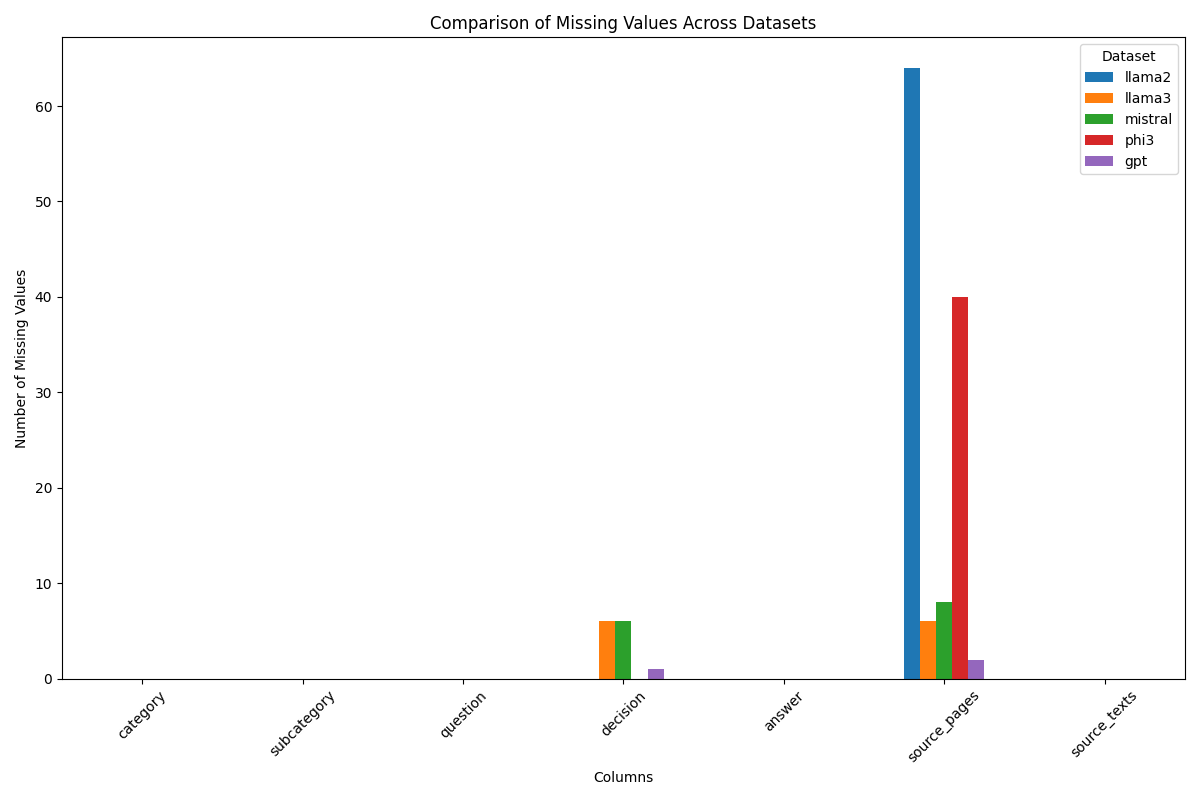
\includegraphics[width=0.8\textwidth]{./images/Missing_Values.png}
    \caption{Comparison of Missing Values Across Models}
    \label{fig:image_label}
\end{figure}

\textbf{Decision Metrics:} The analysis of decisions reveals a noteworthy pattern in the Llama2 model, 
which consistently responded "yes" to all questions. 
In contrast, the Mistral model demonstrated a nearly balanced response distribution, 
with approximately 50$\%$ of answers being "yes" and 50$\%$ being "no." 
The Llama3 and Phi3 models generated more realistic results, 
aligning more closely with the ground truth responses from the ChatGPT-4o model,
though they still underrepresented "yes" responses. 
Notably, both models leaned toward providing a higher proportion of "no" responses compared to "yes." 
Among them, the Mistral model showed a slightly stronger preference for "no" responses than the Llama3 model.
\newline\newline
An analysis of the missing decision entries for the Llama3 and Mistral models reveals the following patterns: 
in the case of the Llama3 model, three missing decisions are from the "target" category, 
two from the "strategy" category, and one from the "tracking" category. \newline
For the Mistral model, both the "strategy" and "tracking" categories have two missing entries each,
while the "target" and "governance" categories have one missing entry each. Notably, 
both models failed to provide an answer for question 36 and both the ChatGPT-4o and Mistral model failed on question 11.
\newline\newline
\textbf{Source Page Metrics:} The majority of questions with missing source pages from the Llama3, Mistral, and Phi3 models 
fall within the "strategy" and "tracking" categories. 
Both the Llama3 and Mistral models fail to cite source pages for question 36. 
Additionally, Llama3 and Phi3 fail to provide source pages for questions 9, 19, 62, and 49, 
while Mistral and Phi3 fail to cite source pages for questions 34, 50, 37, and 63. Notably, 
there is no question for which all three models fail to provide a source page.
\newline\newline
\textbf{Disclosed indicators:} 
When comparing the "yes" and "no" counts of each model across various categories, 
Llama3 and Phi3 exhibit overall similarities. However, 
a closer examination of their counts within subcategories uncovers subtle differences, 
particularly in the distribution of "yes" responses, while "no" responses remain relatively 
consistent between the two models. A similar observation applies to the comparison between Llama3 and ChatGPT-4o.
\newline\newline

\textbf{Semantic Similarity:} 
In this section, we compare the generated answers to the ground truth responses from the ChatGPT-4o model using a LLM-based metric that relies on cosine simularity.  

We begin by comparing the number of questions where each model achieved the highest score. Llama3 dominates with 53 questions, 
followed by Mistral with 5, Llama2 with 4, and Phi3 with 2.

\begin{figure}[H]
    \centering
    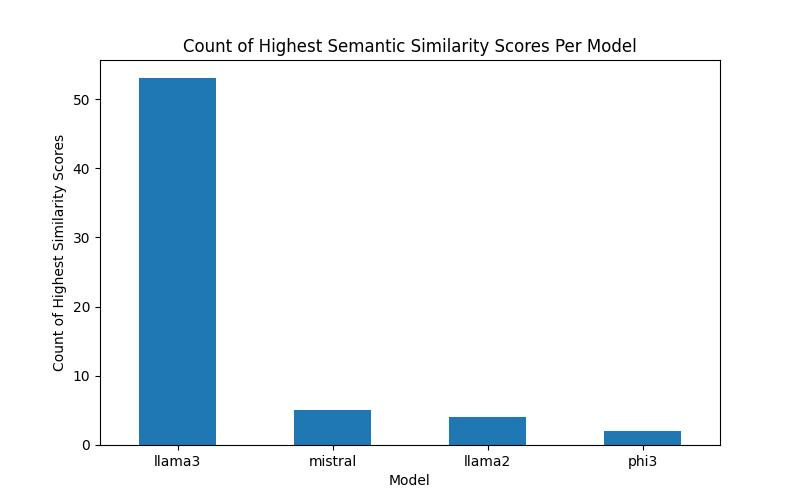
\includegraphics[width=0.6\textwidth]{./images/highest_count_zara.jpg}
    \caption{Most similar response count}
    \label{fig:image_label}
\end{figure}

Furthermore, Llama3 also ranks highest in average similarity, achieving $85\%$ average similarity. This is followed by Mistral at $81.6\%$, Llama2 at $81\%$, and finally, Phi3 at $79\%$.

\begin{center}
    \begin{tabular}{||c c||} 
     \hline
     \textbf{Model} & \textbf{Average Simularity (LLM)}  \\ [0.5ex] 
     \hline
     Llama3 & 0.852544\\ 
     \hline
     Mistral & 0.816881\\ 
     \hline
     Llama2 & 0.810437 \\
     \hline
     Phi3 & 0.798742\\
     \hline
    \end{tabular}
\end{center}

\textbf{Faithfulness:}
Surprisingly, Llama2 achieves the highest faithfulness score, with 58 questions classified as faithful. 
Llama3 comes next with 50, closely trailing Mistral, while Phi3 ranks last with just over 35.
\begin{figure}[H]
    \centering
    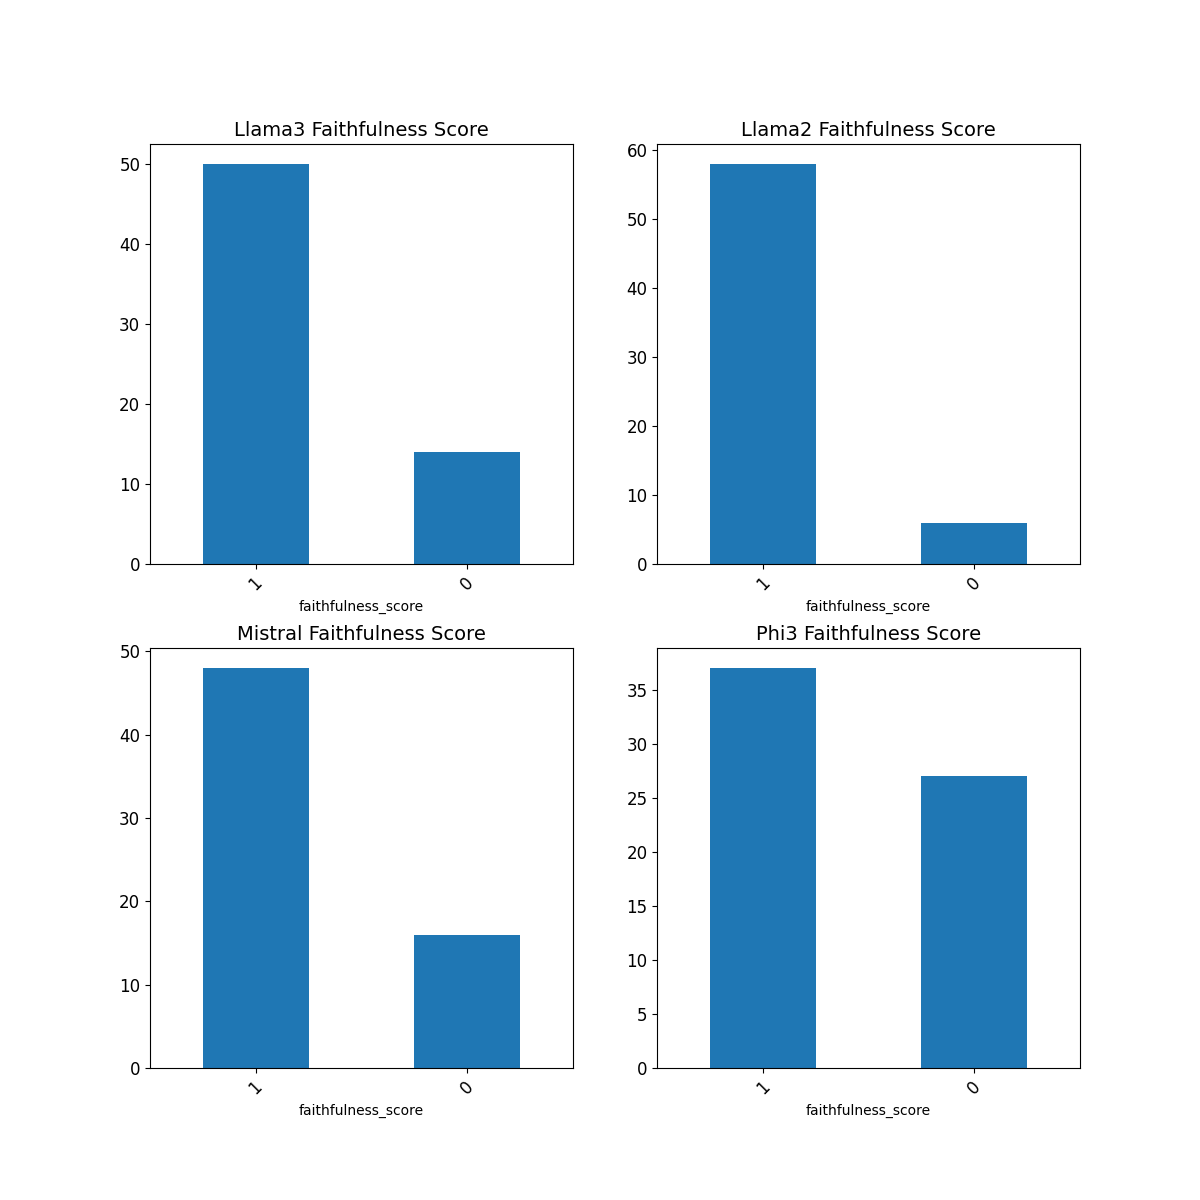
\includegraphics[width=0.8\textwidth]{./images/faith_zara.png}
    \caption{Faithfulness scores}
    \label{fig:image_label}
\end{figure}


\textbf{Correctness:}
Llama3 emerges as the clear winner, with all scores being either 4 or 4.5, and the highest number of 4.5 ratings. Phi3 and Mistral perform similarly, though Phi3 demonstrates greater consistency. 
Llama2 ranks the lowest, with the fewest 4.0 scores and a higher occurrence of lower ratings.
\begin{figure}[H]
    \centering
    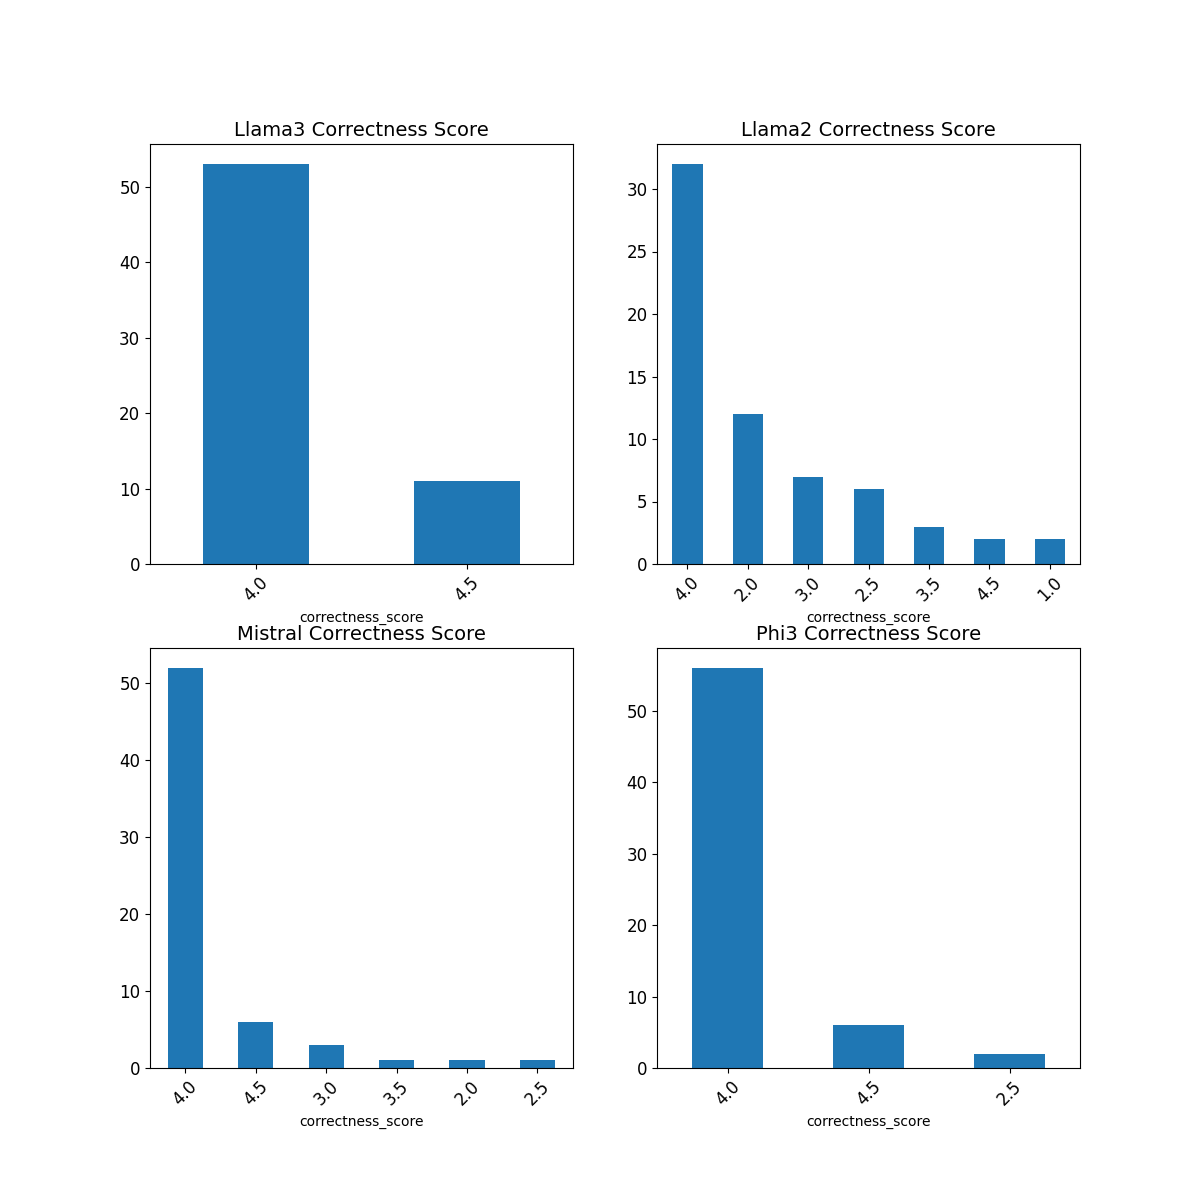
\includegraphics[width=0.8\textwidth]{./images/correct_zara.png}
    \caption{Correctness scores}
    \label{fig:image_label}
\end{figure}

\subsubsection{H$\&$M}
\textbf{Missing Data:} An analysis of the $H\&M$ missing responses shows that the Mistral model failed to answer 
five questions. Similar to the Zara report, 
all models struggled with citing source pages. 
The Llama3 model remained the best-performing in this aspect, with only three missing citations compared to the one missing citation from the ChatGPT-4o model,
while the Llama2 model once again failed to provide any source page citations. 
The Mistral model performed worse compared to the Zara report, 
with seven missing citations this time. 
The Phi3 model also showed a slight decline, failing to cite source pages for 43 entries.
\newline\newline

\textbf{Decision Metrics:}
Once again, the Llama2 model exclusively answered "yes," 
while the Mistral model maintained an approximately 50\% "yes"-"no" response rate. 
The Llama3 and Phi3 models exhibited response ratios similar to those observed in the Zara report.
Both Llama3 and Phi3 seem to underperform on the amount of yes votes compared to the ground truth model ($\sim$ 10 vs 20).
As before, the "target" category accounted for the highest number of missing decisions.

\begin{figure}[H]
    \centering
    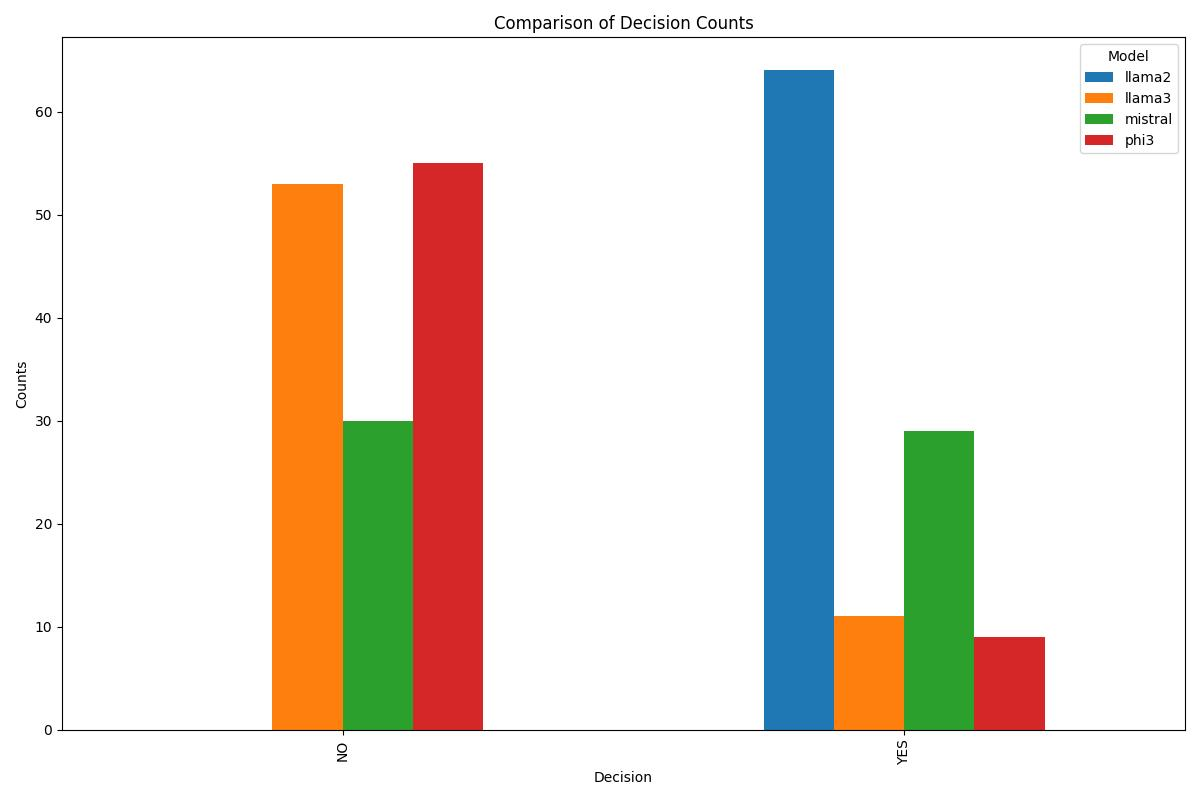
\includegraphics[width=0.8\textwidth]{./images/hm_comparison_decision.jpg}
    \caption{Comparison of Decision Counts Across Models}
    \label{fig:image_label}
\end{figure}

\textbf{Source Page Metrics:} The majority of questions with missing source pages from the Llama3, Mistral, 
and Phi3 models once again fall within the "strategy" and 
"tracking" categories. This time, the Llama3 and Mistral models do not have any overlap in their 
missing source pages. Both Llama3 and Phi3 fail to cite sources for questions 26 and 32, 
while Mistral and Phi3 fail to cite sources for questions 1, 10, 35, and 37. 
Notably, there is still no question for which all three models failed to provide a source page.
\newline\newline

\textbf{Disclosed indicators:} When comparing the "yes"-"no" counts of each model across different categories, 
the counts for Llama3 and Phi3 once again appear to be quite similar overall. However, 
a closer examination within subcategories reveals more pronounced differences compared to the Zara report. 
Meanwhile, the Mistral model continues to maintain an approximately 50-50 response rate across all categories.
\newline\newline

\textbf{Semantic Similarity:} 
Llama3 achieves the highest score with 26 questions, followed by Mistral with 19, Llama2 with 12, and Phi3 with 6.

\begin{figure}[H]
    \centering
    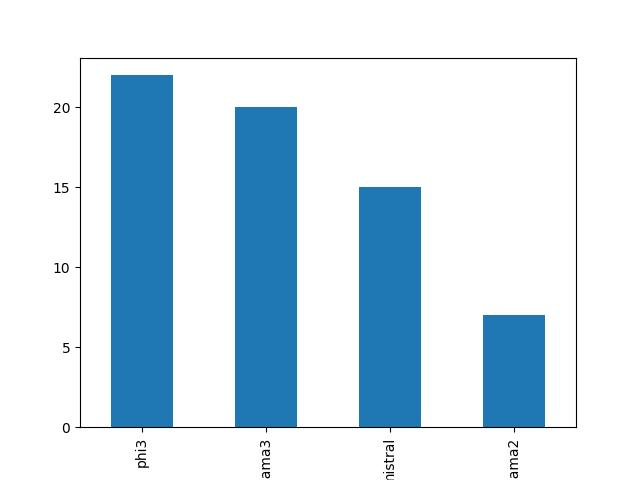
\includegraphics[width=0.6\textwidth]{./images/highest_count_hm.jpg}
    \caption{Most similar response count}
    \label{fig:image_label}
\end{figure}

Additionally, Llama3 leads in average similarity with 80.4\%, followed closely by Mistral at 80\%, Llama2 at 78.8\%, and Phi3 at 78.7\%.

\begin{center}
    \begin{tabular}{||c c||} 
     \hline
     \textbf{Model} & \textbf{Average Simularity (LLM)}  \\ [0.5ex] 
     \hline
     Llama3 &  0.804408\\
     \hline
     Mistral  & 0.800913\\
     \hline
     Llama2 & 0.788172\\
     \hline
     Phi3 &  0.787818 \\
     \hline
    \end{tabular}
\end{center}

\textbf{Faithfulness:}
Phi3 achieves the highest score, followed by Llama3, then Mistral, with Llama2 ranking last.
\begin{figure}[H]
    \centering
    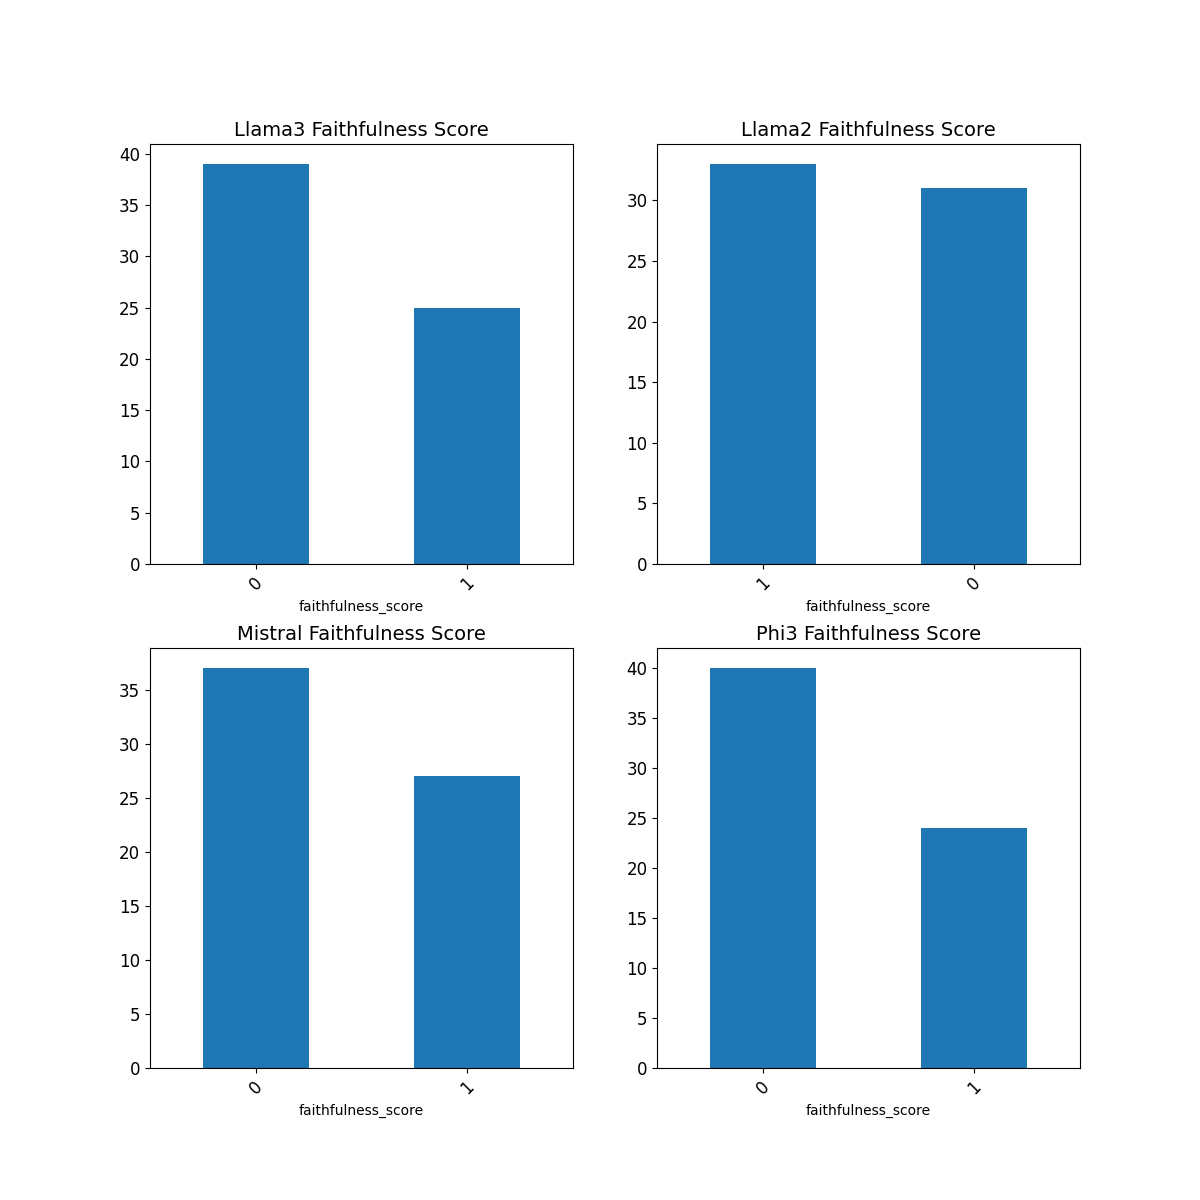
\includegraphics[width=0.8\textwidth]{./images/faith_hm.png}
    \caption{Faithfulness scores}
    \label{fig:image_label}
\end{figure}

\textbf{Correctness:}
Llama3 stands out as the clear winner, delivering the most 4.5 scores and the most consistent answers.  
Phi3 secures second place with the highest number of 4.0 scores, followed by Mistral, while Llama2 ranks last.
\begin{figure}[H]
    \centering
    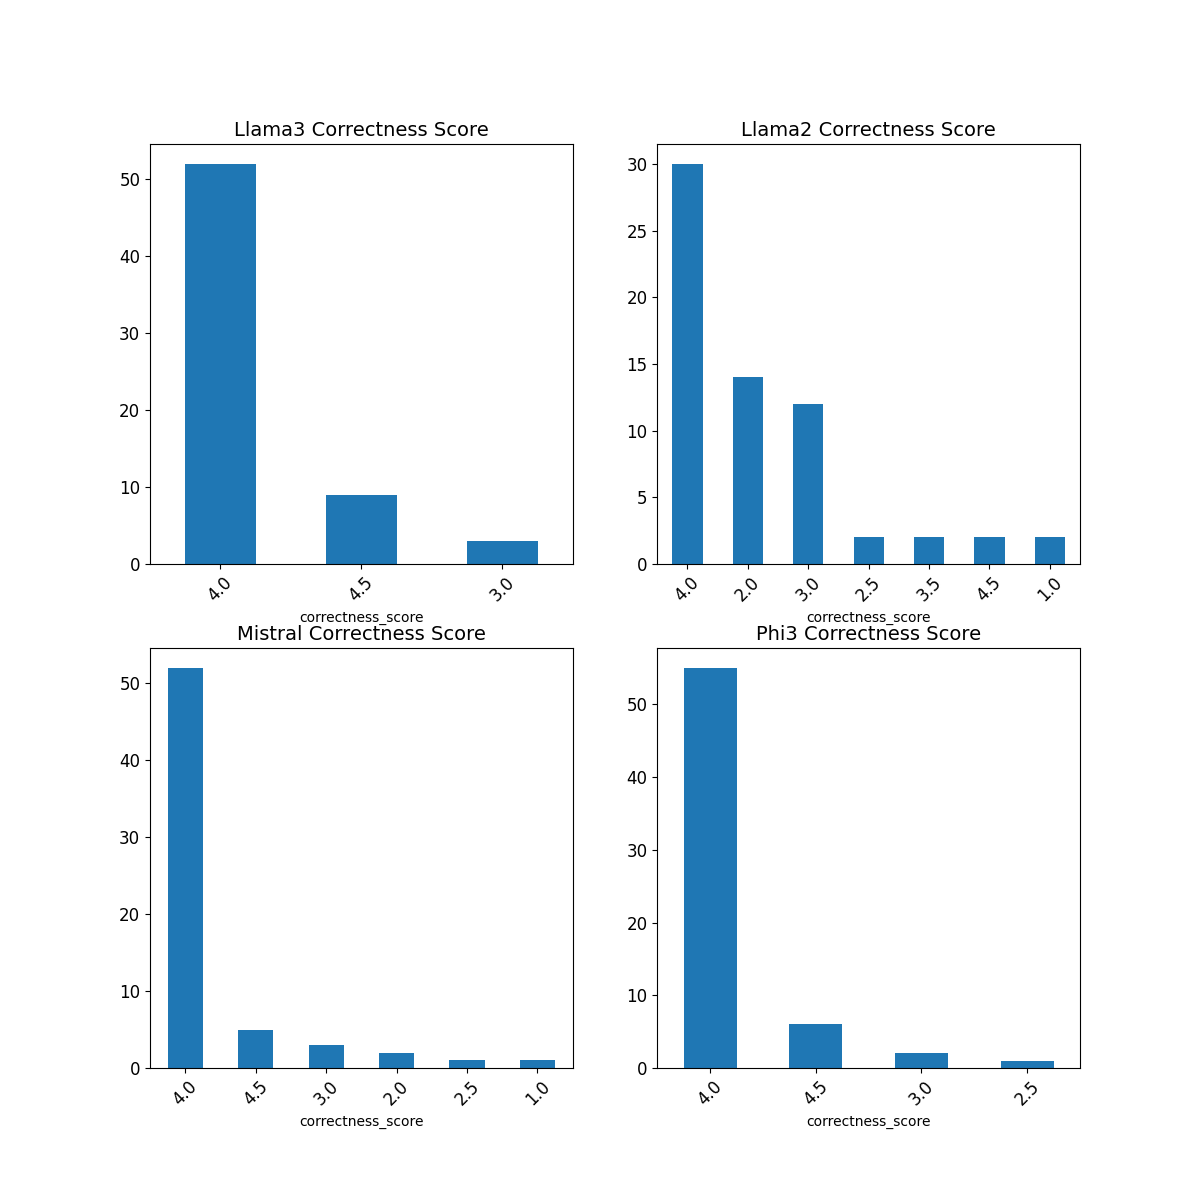
\includegraphics[width=0.8\textwidth]{./images/correct_hm.png}
    \caption{Correctness scores}
    \label{fig:image_label}
\end{figure}
\subsubsection{Context relevancy}
Figure \ref{fig:image_label} shows that the average context relevancy score is higher for Zara than for H\&M, but both scores remain relatively low overall. This suggests that while the Zara report appears to be structured in a way that makes it somewhat easier for the retrieval process to find relevant passages, neither knowledge bases are yielding highly targeted embeddings.
\begin{figure}[H]
    \centering
    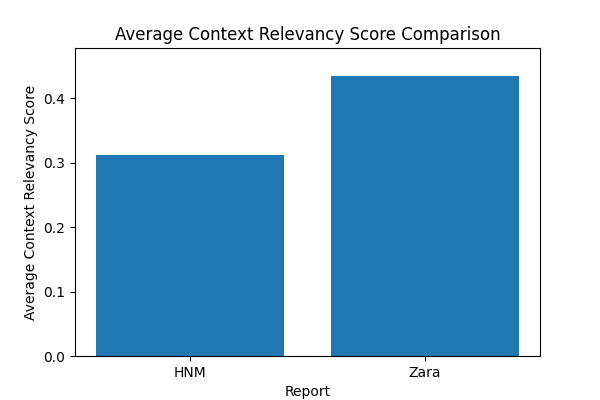
\includegraphics[width=0.8\textwidth]{./images/context_relevancy_comp.png}
    \caption{A comparison of the context relevancy between the Zara and H\&M report}
    \label{fig:image_label}
\end{figure}
\subsection{Scenario Questions}
In this section, we evaluate the models across two scenarios involving custom questions: 
the first scenario consists of 10 questions focused on detecting greenwashing, 
while the second scenario includes 6 questions aimed at addressing greenwashing mitigation.

\subsubsection{Greenwashing Detection}
\textbf{Answer Simularity:} 
For the Zara dataset, Llama3 emerges as the best-performing model, achieving an average cosine similarity of 0.87, followed by Phi3 at 0.82, Llama2 at 0.79, and Mistral at 0.77. Notably, Llama3 outperforms all other models on every question, recording the highest similarity in all nine instances.

In the $H\&M$ dataset, Llama3 again leads with an average similarity score of 0.80, followed by Llama2 at 0.79, Phi3 at 0.78, and Mistral at 0.77. However, unlike the Zara dataset, the distribution of the highest similarity scores is more varied. Llama3 still ranks highest with four questions, while Mistral and Llama2 each achieve the top similarity in two questions, and Phi3 secures one.

These results indicate that Llama3 consistently outperforms other models across both datasets. Llama2 also demonstrates strong performance, particularly in the $H\&M$ dataset, where it surpasses both Mistral and Phi3.

\begin{table}[H]
    \centering
    \begin{tabular}{lcc}
        \toprule
        \textbf{Model} & \textbf{Zara Mean} & \textbf{H\&M Mean} \\
        \midrule
        Llama3  & 0.8707 & 0.8009 \\
        Llama2  & 0.7940 & 0.7879 \\
        Mistral & 0.7732 & 0.7691 \\
        Phi3    & 0.8226 & 0.7819 \\
        \bottomrule
    \end{tabular}
    \caption{Average Cosine Similarity Scores for Zara and H\&M datasets}
    \label{tab:cosine_similarity}
\end{table}

\textbf{Faithfulness:}
For the Zara dataset, Mistral and Llama2 share the top position, each with six counts of 1 and three counts of 3. In contrast, Llama3 and Phi3 tie for last place, both registering five counts of 0 and four counts of 1.  

For the $H\&M$ dataset, Mistral delivers the best performance with eight counts of 1. Llama2 follows in second place with seven counts of 1 and two counts of 0. Phi3 ranks third with five counts of 1 and four counts of 0, while Llama3 comes last, recording four counts of 1 and five counts of 0.

\begin{figure}[H]
    \centering
    \begin{minipage}{0.49\textwidth}
        \centering
        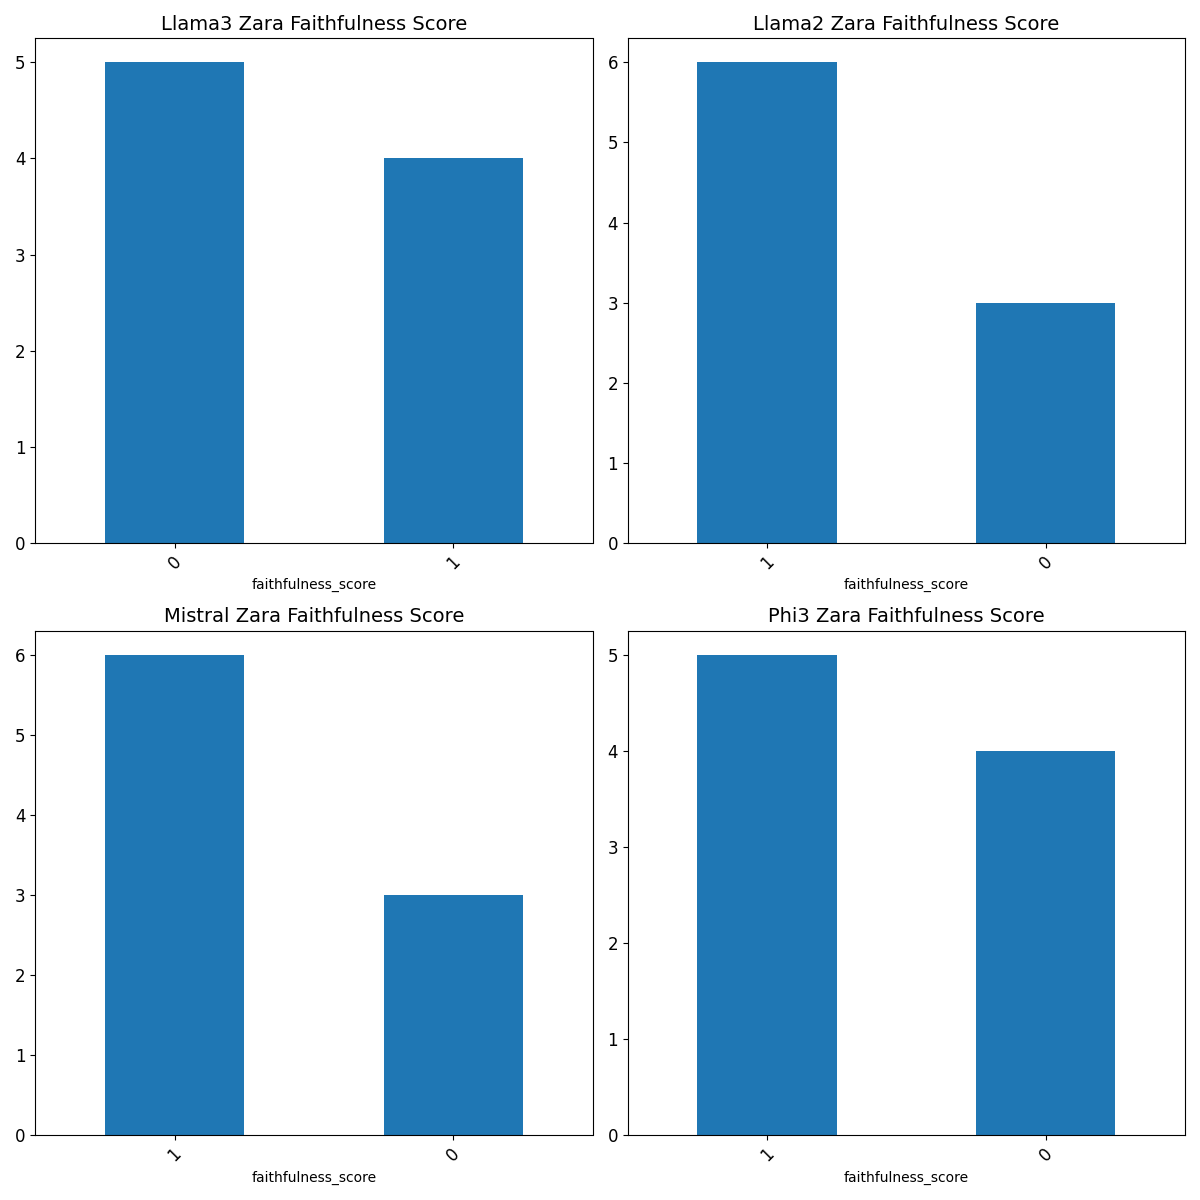
\includegraphics[width=\textwidth]{./images/faith_zara_scene_det.png}
        \caption{Correctness scores Zara}
        \label{fig:faith_zara}
    \end{minipage}
    \hfill
    \begin{minipage}{0.49\textwidth}
        \centering
        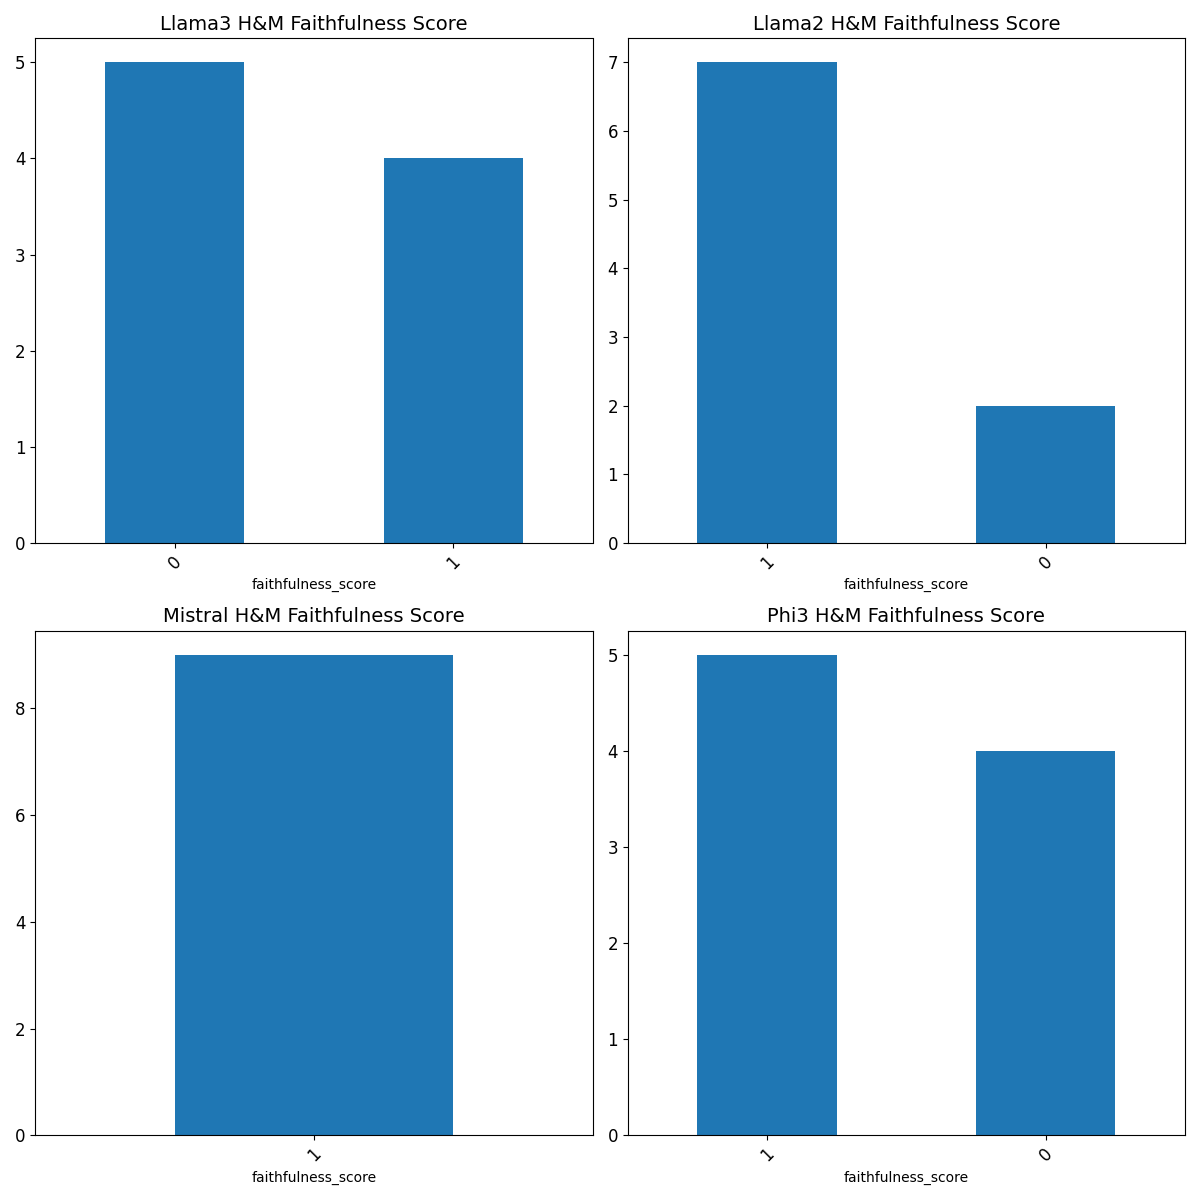
\includegraphics[width=\textwidth]{./images/faith_hm_scene_det.png}
        \caption{Correctness scores $H\&M$}
        \label{fig:faith_hm}
    \end{minipage}
\end{figure}

\textbf{Correctness:}
For the Zara dataset, Llama3 is the only model to achieve a score of 4.5, while all other models score 4.  
For the $H\&M$ dataset, Llama2 is the only model to reach a score of 4.5, while Phi3 and Mistral both score 4. Llama3 performs the worst, with one score of 2 and the rest at 4.

\subsubsection{Greenwashing Mitigation}
\textbf{Answer Simularity:} 
For the greenwashing mitigation on the Zara dataset, Llama2 achieves the highest average similarity score at 0.798, followed closely by Llama3 at 0.788. 
Mistral ranks third with 0.773, while Phi3 has the lowest score at 0.760. In terms of the number of questions with the highest similarity, Llama2 leads with three, followed by Mistral with two and Llama3 with one.

For the $H\&M$ dataset, Llama2 once again secures the highest average similarity score at 0.794, with Mistral close behind at 0.783. Phi3 takes third place with 0.745, while Llama3 has the lowest score at 0.734. 
Interestingly, there is a three-way tie for the most questions with the highest similarity, with Llama3, Llama2, and Mistral each achieving the top score in the same number of instances.

\begin{table}[H]
    \centering
    \begin{tabular}{lcc}
        \toprule
        \textbf{Model} & \textbf{Zara Mean} & \textbf{H\&M Mean} \\
        \midrule
        Llama3  & 0.7881 & 0.7339 \\
        Llama2  & 0.7984 & 0.7936 \\
        Mistral & 0.7731 & 0.7828 \\
        Phi3    & 0.7598 & 0.7449 \\
        \bottomrule
    \end{tabular}
    \caption{Average Cosine Similarity Scores for Greenwashing Mitigation on Zara and H\&M datasets}
    \label{tab:greenwashing_mitigation}
\end{table}

\textbf{Faithfulness:}
For the Zara dataset, Llama3 ranks first with five counts of 1, followed by Llama2 in second place with four counts of 1. Mistral and Phi3 share the last position, each with three counts of 1.  

In the $H\&M$ dataset, the ranking remains similar, but this time, Llama3 and Llama2 tie for first place, while Mistral and Phi3 once again share the last position.
\begin{figure}[H]
    \centering
    \begin{minipage}{0.49\textwidth}
        \centering
        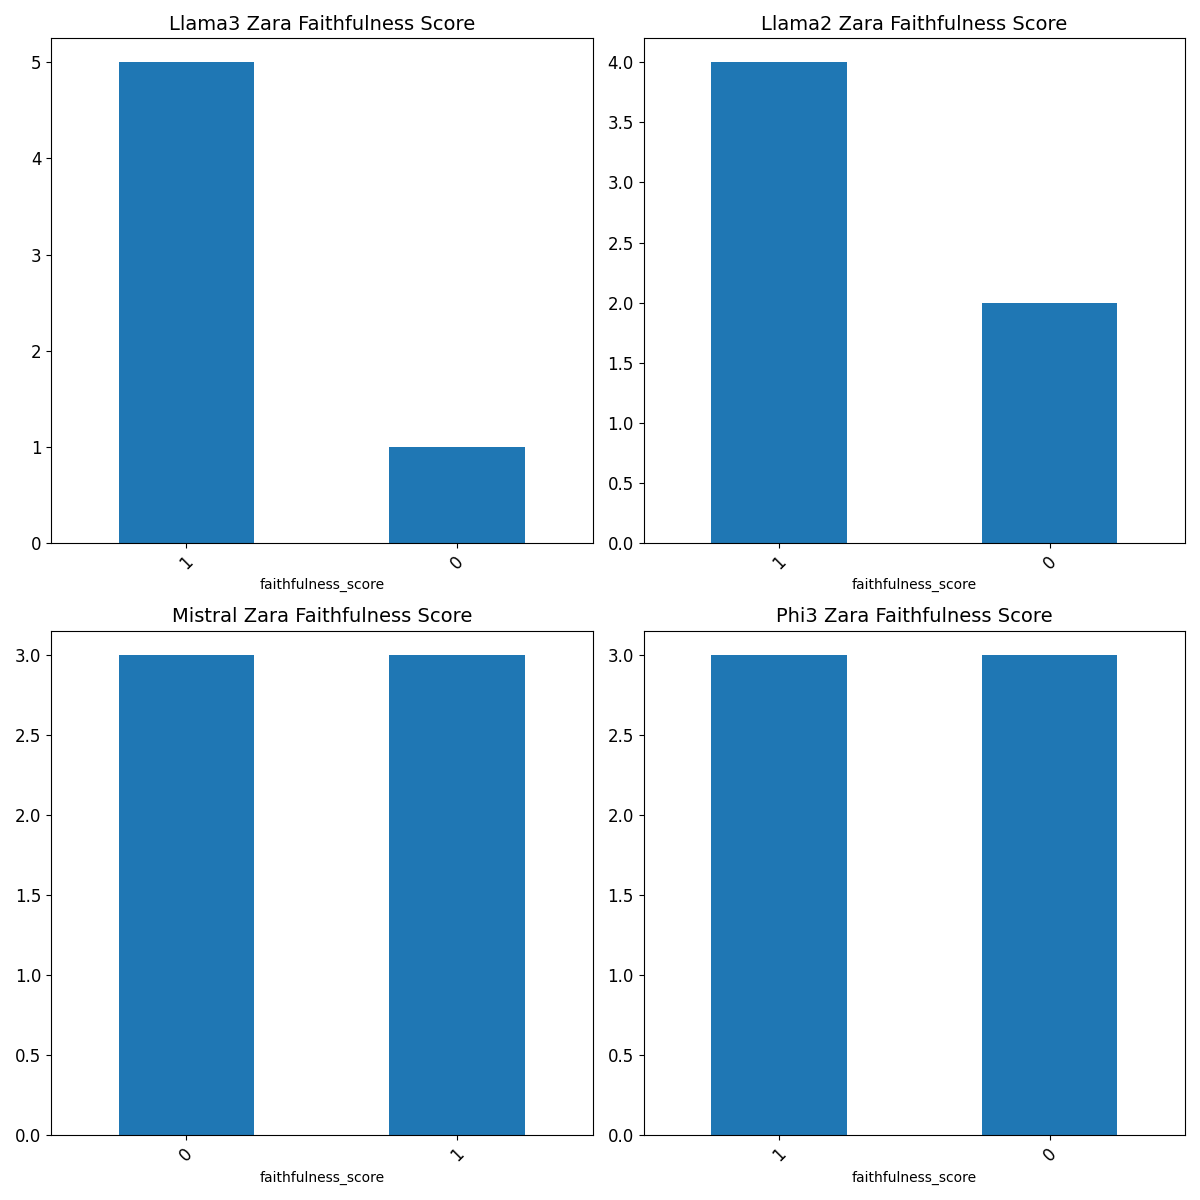
\includegraphics[width=\textwidth]{./images/faith_zara_scene_mit.png}
        \caption{Correctness scores Zara}
        \label{fig:faith_zara}
    \end{minipage}
    \hfill
    \begin{minipage}{0.49\textwidth}
        \centering
        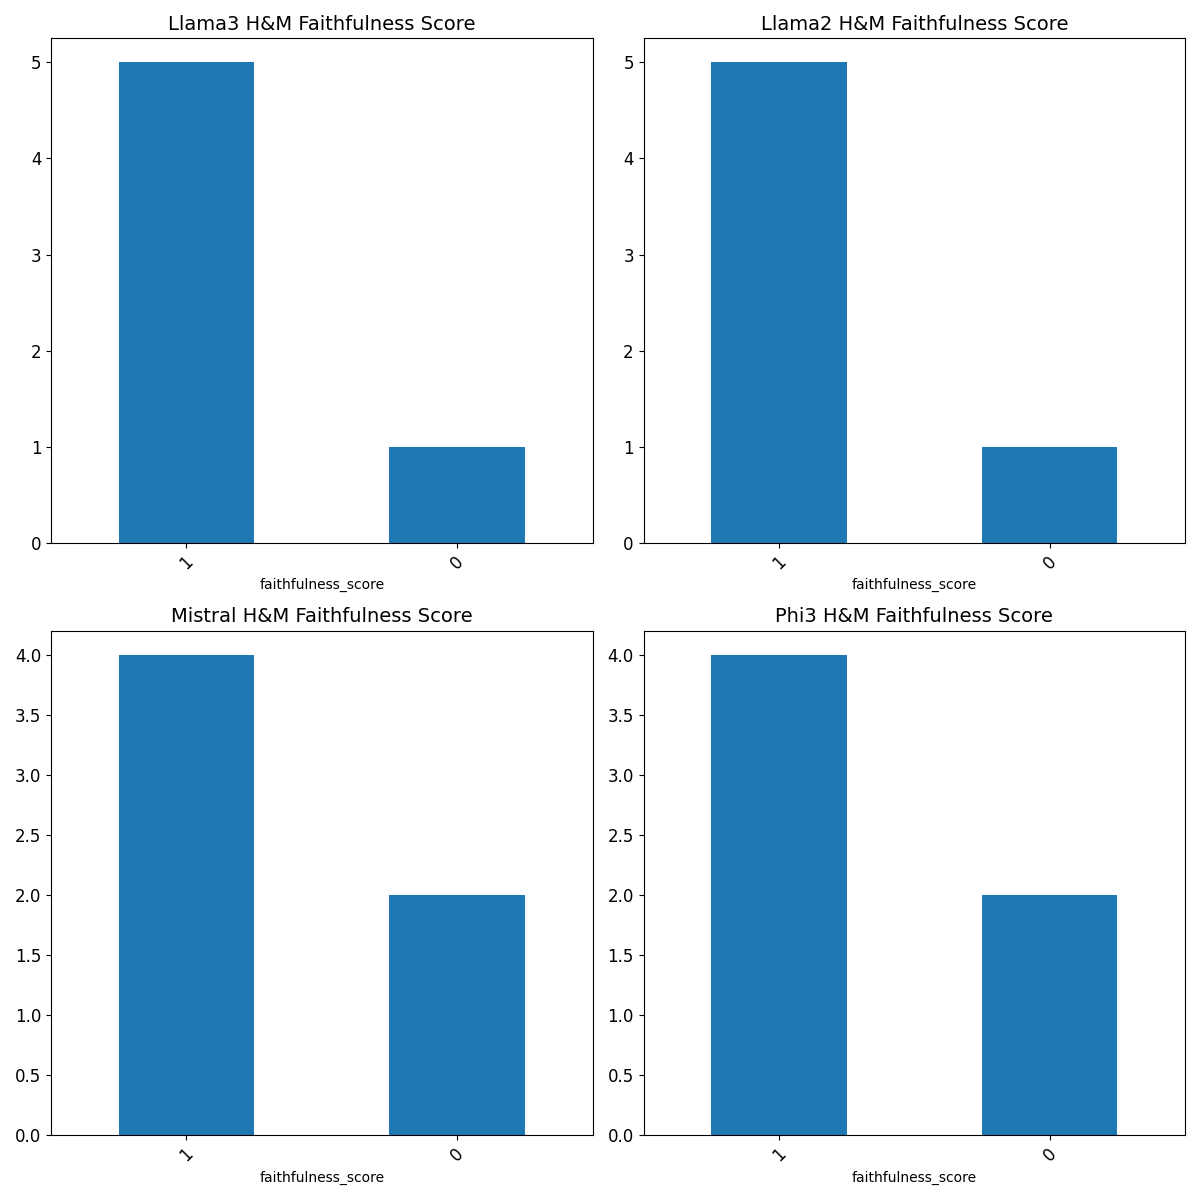
\includegraphics[width=\textwidth]{./images/faith_hm_scene_mit.png}
        \caption{Correctness scores $H\&M$}
        \label{fig:faith_hm}
    \end{minipage}
\end{figure}

\textbf{Correctness:}
In the Zara dataset, Llama3 is the only model to achieve a score of 4.5. Both Mistral and Llama2 score 4, while Phi3 performs the worst, with only four instances of a score of 4 and lower consistency compared to Llama2 and Mistral.  
For the $H\&M$ dataset, Llama2 is the only model to achieve a 4.5. Mistral follows in second place with six instances of a score of 4. Phi3 outperforms Llama3 with one additional score of 4 and greater consistency.

\subsection{Conclusion}
The evaluation and results highlight notable trends and differences across the four models when applied to both the Zara and $H\&M$ datasets, 
as well as to the custom scenarios of greenwashing detection and mitigation.

Llama3 consistently emerges as the strongest performer overall in terms of answer similarity, 
achieving the highest average similarity scores and the highest count of questions most similar to the ChatGPT-4o ground truth.
Phi3 also demonstrates strong performance, often ranking second in both metrics. 
However, Phi3’s performance in citing source pages remains a significant challenge. Mistral provides balanced decision-making and leads in some scenario-specific evaluations,
such as greenwashing detection for $H\&M$, but it lags behind in citation completeness and average similarity scores. Llama2, while consistent in its "yes" responses, continues to struggle significantly with citing source pages, realistic decision-making, and overall similarity performance.

In the greenwashing detection scenario, Llama3 achieved the highest average semantic similarity scores for both the Zara and $H\&M$ datasets, with 87\% and 80\%, respectively. It also dominated in overall similarity, attaining the highest similarity score in all 9 questions for the Zara dataset and in 4 questions for the $H\&M$ dataset.  
Phi3 also performed well in terms of average similarity, scoring 82\% for the Zara dataset, but slightly lower at 78\% for the $H\&M$ dataset. Meanwhile, Llama2 and Mistral demonstrated strong performance in the faithfulness evaluation.

In the greenwashing mitigation scenario, Llama2 achieved the highest average similarity scores and the highest number of questions with the highest similarity for both the Zara and $H\&M$ datasets.  
For the correctness metric, Llama3 performed slightly better than Llama2 in the Zara dataset but was surpassed by Llama2 in the $H\&M$ dataset.  
Llama3 also demonstrated the strongest performance in the faithfulness metric for both datasets. However, in the $H\&M$ dataset, it tied with Llama2.

Across both datasets and scenarios, the majority of missing source pages remain concentrated in the "strategy" and "tracking" categories, highlighting a common area for improvement across all models. 
While Llama3 and Mistral show overlapping weaknesses on specific questions, such as question 36 in the Zara dataset, no single question consistently failed across all models.

Overall, while Llama3 maintains its position as the leading model in most evaluations, Phi3 demonstrates scenario-specific strengths. 
Mistral provides balanced decision-making and stands out in some detection tasks but needs refinement in citation and overall consistency. 
Llama2 performed above expectations in the greenwashing mitigation scenario but is severaly lacking in the decision making and citation aspect.

\subsection{Ethical considerations}

In this section, we discuss some ethical considerations.
In the setup we used, we ask LLM models to judge whether questions are true or false, and to provide argumentation about the decision made.
In the argumentation, the LLM model must refer to the source chunks that were used to base the decision on.
Therefore, this solution is reasonably \textbf{transparant} and \textbf{explainable}, as it provides insight in how a decision was made by quoting the relevant information.
However, this does not necessarily imply \textbf{trustworthiness}.
The authors of \cite{durability} warned that the RAG solution could generate valuable output but should not be seen as a replacement for human experts.
Furthermore, as we are comparing the answers to ground truth values produced by ChatGPT-4o, we can only have faith in the produced answers and metrics if we trust the ground truths to be accurate.
There is a degree of \textbf{input bias} in our experiments.
Companies have a vested interest in publishing optimistic and forward-looking sustainability reports.
In other words, the reports used to provide argumentation to the questions answered, are not necessarily objective.
Furthermore, since ChatGPT was used to establish ground truths for the questions, any and all biases present in that model would leak in the performance metrics.
Finally, \textbf{regulation} is important in this context as well.
On the one hand, there is already regulation requiring companies to publish sustainability reports.
On the other hand, more regulation could be necessary to assure the reports are trustworthy and legally binding.

\section{Conclusions and Discussion} \label{sec:conclusions}

For this assignment, we have adapted the approach described in \cite{durability} to evaluate questions related to greenwashing on fast fashion durability reports.
Instead of relying on a single closed source LLM, we have evaluated four open source models (\texttt{Llama2}, \texttt{Llama3:instruct}, \texttt{Mistral} and \texttt{phi3:14b-instruct}).
To evaluate the performance of these models, we have used several metrics (faithfulness, context relevancy, correctness, semantic similarity).

The main conclusions of this research are : \textbf{i)} all evaluated models exhibit poor performance in the classification of indicators, with some models consistently selecting a single class and others appearing to choose classes at random, which indicates the models lack real reasoning, \textbf{ii)} generating source page citations proves to be highly challenging for the models and \textbf{iii)} semantic similarity between the model output and the ground truth is reasonable, but the other metrics show important differences between the models tested and ChatGPT-4o.
The \texttt{Llama2} model - the smallest LLM model we tested -  consistently scores worst.
The \texttt{Llama3:instruct} model seems to perform best.
The instruction tuning done for this model appears to help for these specific tasks.
Against our expectations, the instruction tuned \texttt{Phi3:14b-instruct} model is almost twice the size of \texttt{Llama3:instruct}, but performs consistently worse than the latter.
Even though the RAG setup permits answering domain specific questions by introducing the right context, we clearly see the limitations of such a setup as well.
Introducing the right context alone is not sufficient to coherently and accurately answer questions that need reasoning about that context.

We see several opportunities for future research.
First, the setup we introduced permits to use any model available for Ollama.
It would be interesting to test more powerful models that contain more weights and are specifically trained for reasoning, such as Deepseek.
Due to hardware constraints, we were unable to perform the tests on more advanced models.
Second, a supervised finetuning approach of one or more of the models we tested could be performed.
In particular, the models could be finetuned to accommodate answering the type of questions used in this assignment.
Third, the architecture of the setup could be improved.
The retriever of a RAG setup is a crucial part that heavily influences performance of the entire solution.
Tests can be done using other embedding models, other hyperparameters to populate the vector store, and other retriever components.

This assignment fits in the cluster of \textbf{text} of the Capita Selecta in Artificial Intelligence course organised by the Open University (\cite{ou}).
In this cluster, a number of techniques are studied that try to remedy some of the most important shortcomings of LLM models (training and inference cost, no domain specific knowledge, cutoff of knowledge, etc).
This research used an RAG setup to introduce domain specific knowledge, bypass any cutoff of knowledge and to generate more diverse and factual answers.
The setup proved successful in augmenting the capabilities of (older) LLM models, but unsuccessful in letting the models reason about the questions we asked.

\printbibliography

\end{document}
